\documentclass[a4paper]{article}
\usepackage[utf8]{inputenc}
\usepackage[russian]{babel}
\usepackage{listings}
\usepackage[a4paper,margin=1.in]{geometry}
\usepackage{indentfirst}
\usepackage{graphicx}
\usepackage{caption}
\usepackage{float}

%\setcounter{topnumber}{2}
%\setcounter{bottomnumber}{2}
%\setcounter{totalnumber}{4}
%\renewcommand{\topfraction}{0.85}
%\renewcommand{\bottomfraction}{0.85}
%\renewcommand{\textfraction}{0.15}
%\renewcommand{\floatpagefraction}{0.8}
%\renewcommand{\textfraction}{0.1}
%\setlength{\floatsep}{5pt plus 2pt minus 2pt}
%\setlength{\textfloatsep}{5pt plus 2pt minus 2pt}
%\setlength{\intextsep}{5pt plus 2pt minus 2pt}

\begin{document}

\title{Сравнение вращаемой и сдвиговой множественных развёрток по количеству вычислений целевой функции в задачах без ограничений}
\author{}
\date{}
\maketitle

\section{Реализация алгоритма с множественными развёртками}
Алгоритм реализован на языке C++ с использованием линейных структур данных для хранения поисковой информации.
Сложность выполнения каждой итерации алгоритма $O(k)$, где $k$ --- номер итерации.

Реализация поддерживает полноценную индексную схему, $\varepsilon$-резервирование и локальную адаптацию (схема Маркина-Стронгина).
Поддержки параллельных вычислений нет.

Данная реализация не использует код системы Globalizer.

\section{Классы тестовых задач и методика проведения экспериментов}

Операционные характеристики метода с различными множественнными развёртками сторились на следующих классах задач:
функции Гришагина ($F_{GR}$), GKLS 2d Simple (gklsS2d), GKLS 2d Hard (gklsH2d), GKLS 3d Simple (gklsS3d).

Для каждого класса задач и каждого типа развёртки были предприняты попытки провести следующие эксперименты:
\begin{enumerate}
  \item решить все задачи при одинаковом для всех развёрток значении $r$ с остановкой по попаданию в окрестность известного оптимума;
  \item решить все задачи при одинаковом для всех развёрток значении $r$ с остановкой по точности;
  \item решить все задачи при минимальном допустимом для каждой конфигурации развёртки в отдельности значении параметра $r$ с остановкой по попаданию в окрестность известного оптимума;
  \item решить все задачи при минимальном допустимом для каждой конфигурации развёртки в отдельности значении параметра $r$ с остановкой по точности;
\end{enumerate}

В последних двух случаях подбор минимального значения $r$ такого, что решаются все задачи класса, осуществлялся с точностью 0.1 для каждого типа
развёртки в отдельности и для каждого значения $L$ (количество развёрток).

В связи с тем, что в представленной реализации АГП используются только линейные структуры данных, не для всех классов указанные 4 типа эспериментов были проведены. Решение некоторых задач из сложных классов требует порядка $10^6$ испытаний и занимает несколько часов на одну задачу. В этом случае подобрать минимальное значение $r$ для каждой развёртки очень затратно.

В таблицах \ref{table:exp1}, \ref{table:exp2}, \ref{table:exp3}, \ref{table:exp4} указаны эксперименты, которые были проведены. Каждый эксперимент включает в себя решение всех задач класса при $l=1,2,3$ для вращаемой развёртки и
$l=1,2,3,4$ для сдвиговой.

\begin{table}
\begin{center}
\caption{Эксперименты, проведённые при минимальном значении $r$ с остановкой по попаданию в окрестность оптимума}
  \begin{tabular}{l|l*{4}{c}r}
    \label{table:exp1}
  Тип развёртки & $F_{GR}$ & gklsS2d & gklsH2d & gklsS3d \\
  \hline
  вращаемая, $L=1$ & + & + & + & + \\
  вращаемая, $L=2$ & + & + & + & + \\
  вращаемая, $L=3$ & + & + & + & + \\
  сдвиговая, $L=1$ & + & + & + & + \\
  сдвиговая, $L=2$ & + & + & + & + \\
  сдвиговая, $L=3$ & + & + & + & + \\
  сдвиговая, $L=4$ & + & + & - & - \\
  \end{tabular}
\end{center}
\end{table}

\begin{table}
\begin{center}
\caption{Эксперименты, проведённые при минимальном значении $r$ с остановкой по точности}
  \begin{tabular}{l|l*{4}{c}r}
    \label{table:exp2}
  Тип развёртки & $F_{GR}$ & gklsS2d & gklsH2d & gklsS3d \\
  \hline
  вращаемая, $L=1$ & + & + & + & - \\
  вращаемая, $L=2$ & + & + & + & - \\
  вращаемая, $L=3$ & + & + & - & - \\
  сдвиговая, $L=1$ & + & + & + & - \\
  сдвиговая, $L=2$ & + & + & - & - \\
  сдвиговая, $L=3$ & + & + & - & - \\
  сдвиговая, $L=4$ & + & + & - & - \\
  \end{tabular}
\end{center}
\end{table}

\begin{table}
\begin{center}
\caption{Эксперименты, проведённые при одинаковом значении $r$ с остановкой по попаданию в окрестность оптимума}
  \begin{tabular}{l|l*{4}{c}r}
    \label{table:exp3}
  Тип развёртки & $F_{GR}$ & gklsS2d & gklsH2d & gklsS3d \\
  \hline
  вращаемая, $L=1$ & + & + & + & + \\
  вращаемая, $L=2$ & + & + & + & + \\
  вращаемая, $L=3$ & + & + & + & + \\
  сдвиговая, $L=1$ & + & + & + & + \\
  сдвиговая, $L=2$ & + & + & + & + \\
  сдвиговая, $L=3$ & + & + & + & + \\
  сдвиговая, $L=4$ & + & + & - & - \\
  \end{tabular}
\end{center}
\end{table}

\begin{table}
\begin{center}
\caption{Эксперименты, проведённые при одинаковом значении $r$ с остановкой по точности}
  \begin{tabular}{l|l*{4}{c}r}
    \label{table:exp4}
  Тип развёртки & $F_{GR}$ & gklsS2d & gklsH2d & gklsS3d \\
  \hline
  вращаемая, $L=1$ & + & + & + & + \\
  вращаемая, $L=2$ & + & + & + & + \\
  вращаемая, $L=3$ & + & + & - & - \\
  сдвиговая, $L=1$ & + & + & + & + \\
  сдвиговая, $L=2$ & + & + & - & - \\
  сдвиговая, $L=3$ & + & + & - & - \\
  сдвиговая, $L=4$ & + & + & - & - \\
  \end{tabular}
\end{center}
\end{table}

Во всех экспериментах с остановкой по попаданию в окрестность глобального минимума использовалось значение
$\varepsilon=10^{-2}$. При остановке по точности $\varepsilon \in [10^{-3};5\cdot 10^{-3}]$ в зависимости от класса задач.
Также в некоторых случаях для ограничения, порождаемого сдвиговой развёрткой, использовалось $\varepsilon$-резервирование
величиной 0.05. Для сложных классов был задействован смешанный локально-глобальный алгоритм с параметром смешивания $q=4$.

\subsection{Опeрационные характеристики}
Операционные характеристики были построены практически для всех столбцов таблиц из предыдущего раздела.
В случае сдвиговой развёртки наличие дополнительного ограничения не учитывались при построении операционных характеристик.
\subsubsection{Класс $F_{GR}$}

\begin{figure}
  \center
  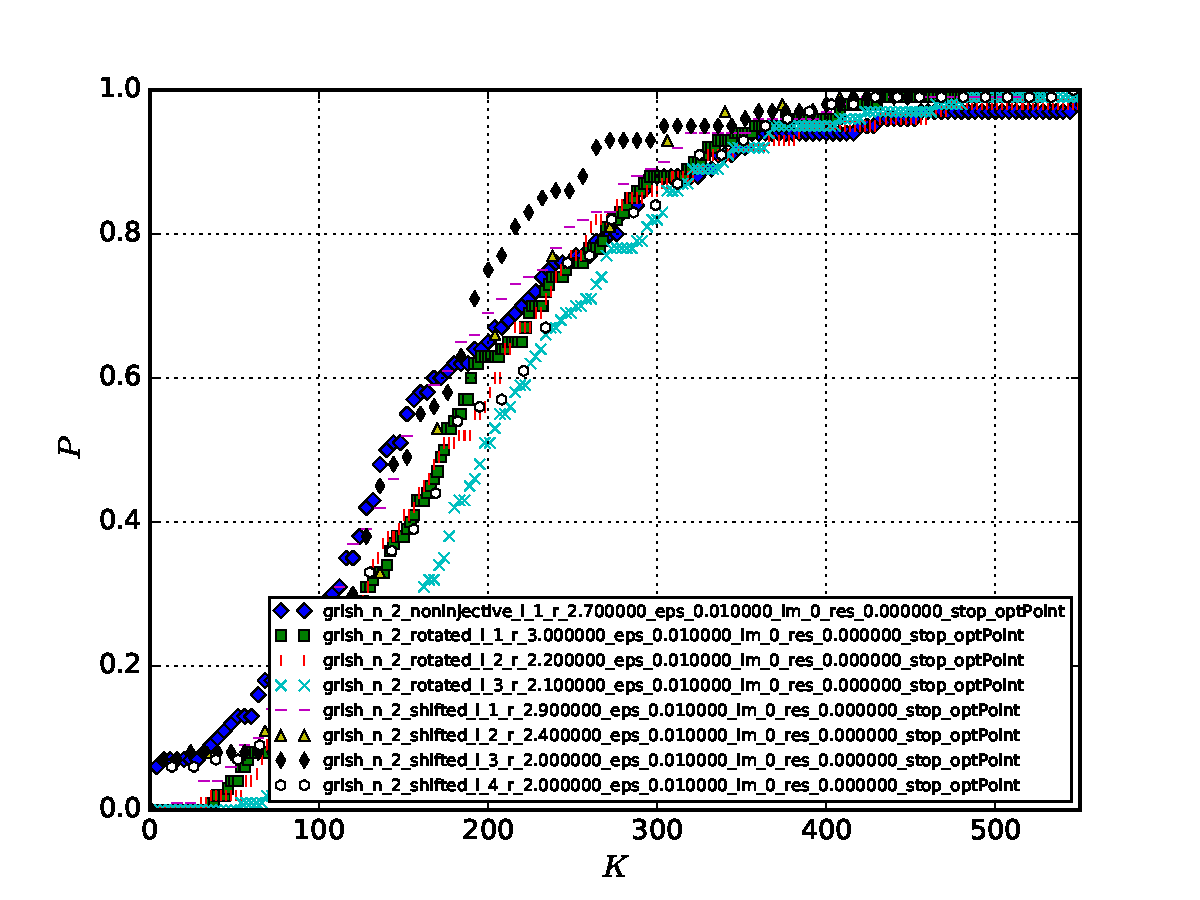
\includegraphics[width=0.95\textwidth]{../f_gr/opt_point/grish_opt_point_op.pdf}
  \caption{$F_{GR}$, остановка по попаданию в окрестность, минимальное значение $r$}
  \label{fig:}
\end{figure}

\begin{figure}[H]
  \center
  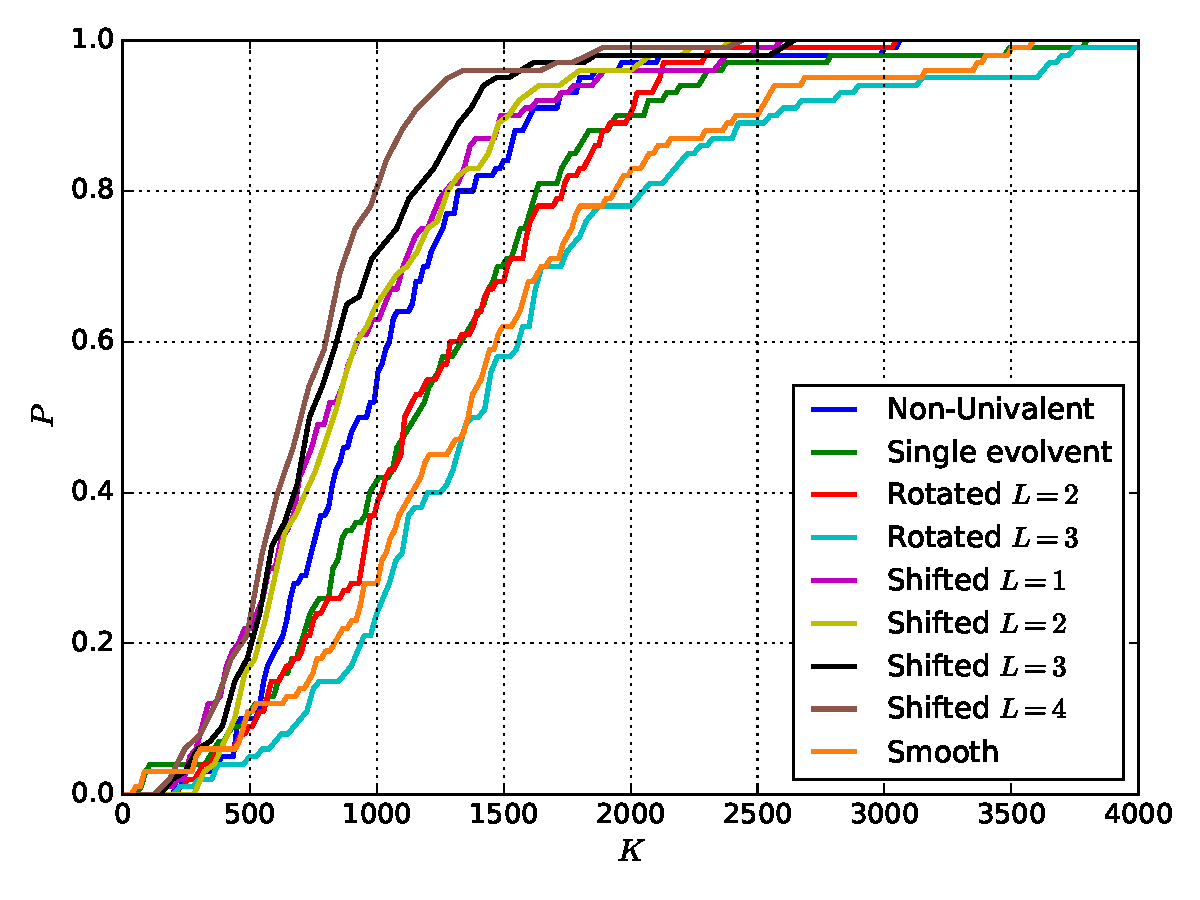
\includegraphics[width=0.95\textwidth]{../f_gr/accuracy/grish_accur_op.pdf}
  \caption{$F_{GR}$, остановка по точности, минимальное значение $r$}
  \label{fig:}
\end{figure}

\begin{figure}[H]
  \center
  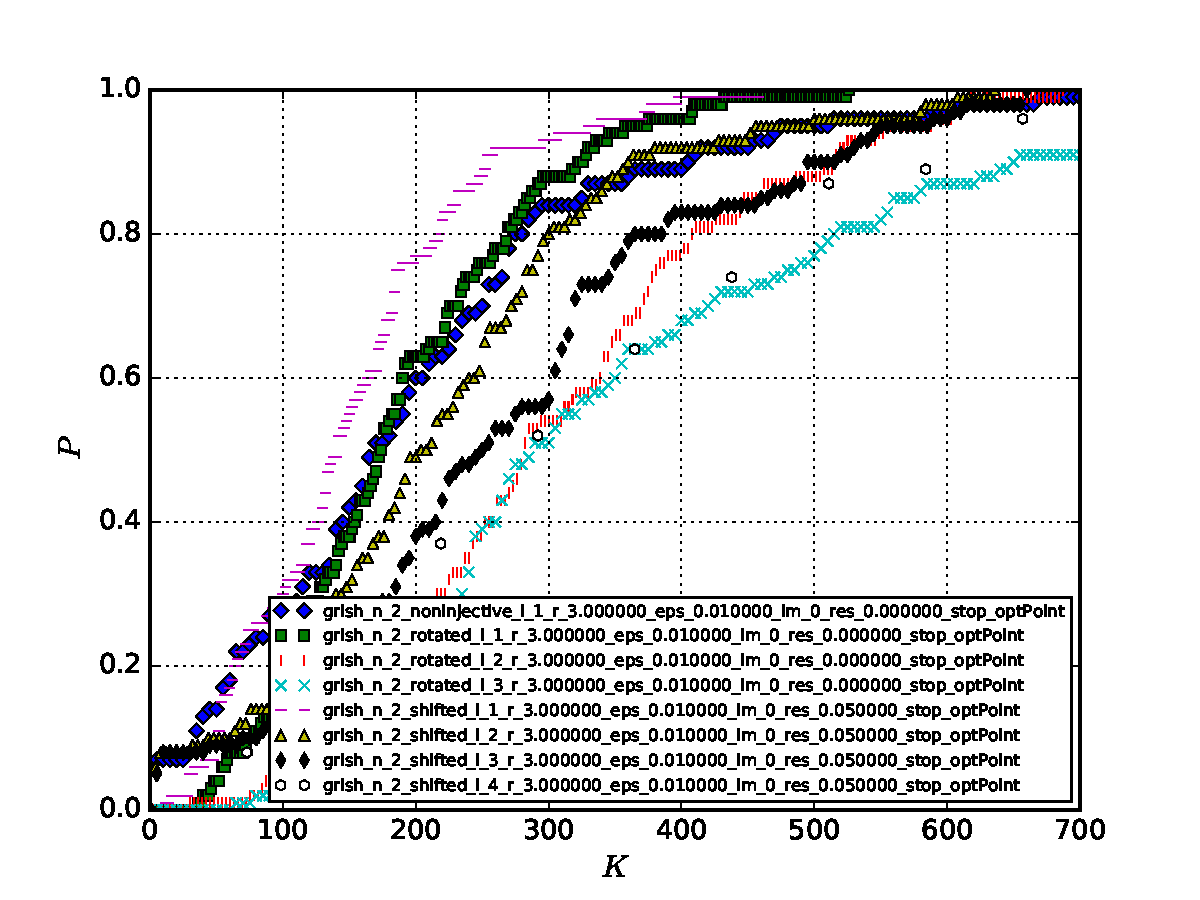
\includegraphics[width=0.95\textwidth]{../f_gr/same_r/opt_point/grish_same_r_opt_point.pdf}
  \caption{$F_{GR}$, остановка по попаданию в окрестность, $r=3.0$}
  \label{fig:}
\end{figure}

\begin{figure}[H]
  \center
  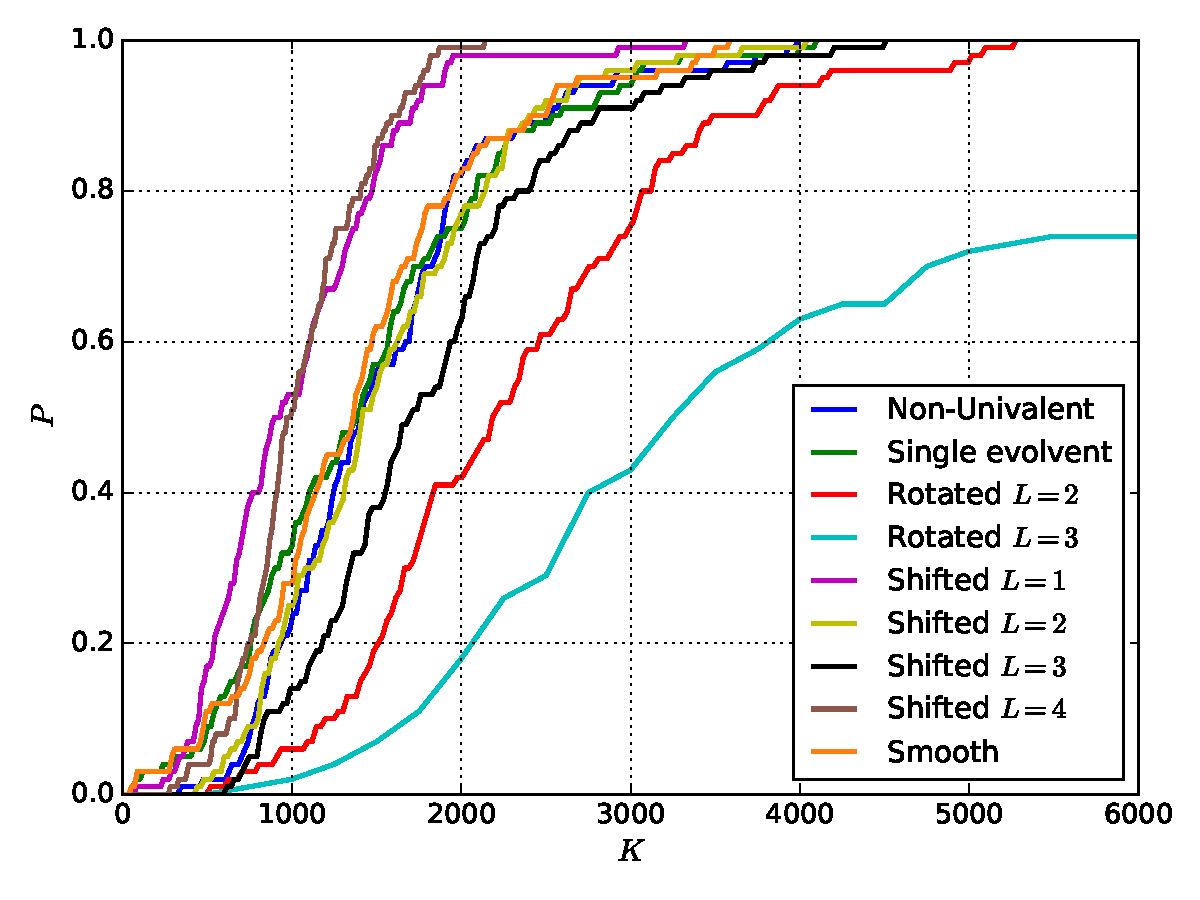
\includegraphics[width=0.95\textwidth]{../f_gr/same_r/accuracy/grish_same_r_acc.pdf}
  \caption{$F_{GR}$, остановка по точности, $r=3.1$}
  \label{fig:}
\end{figure}

\subsubsection{Класс gklsS2d}

\begin{figure}
  \center
  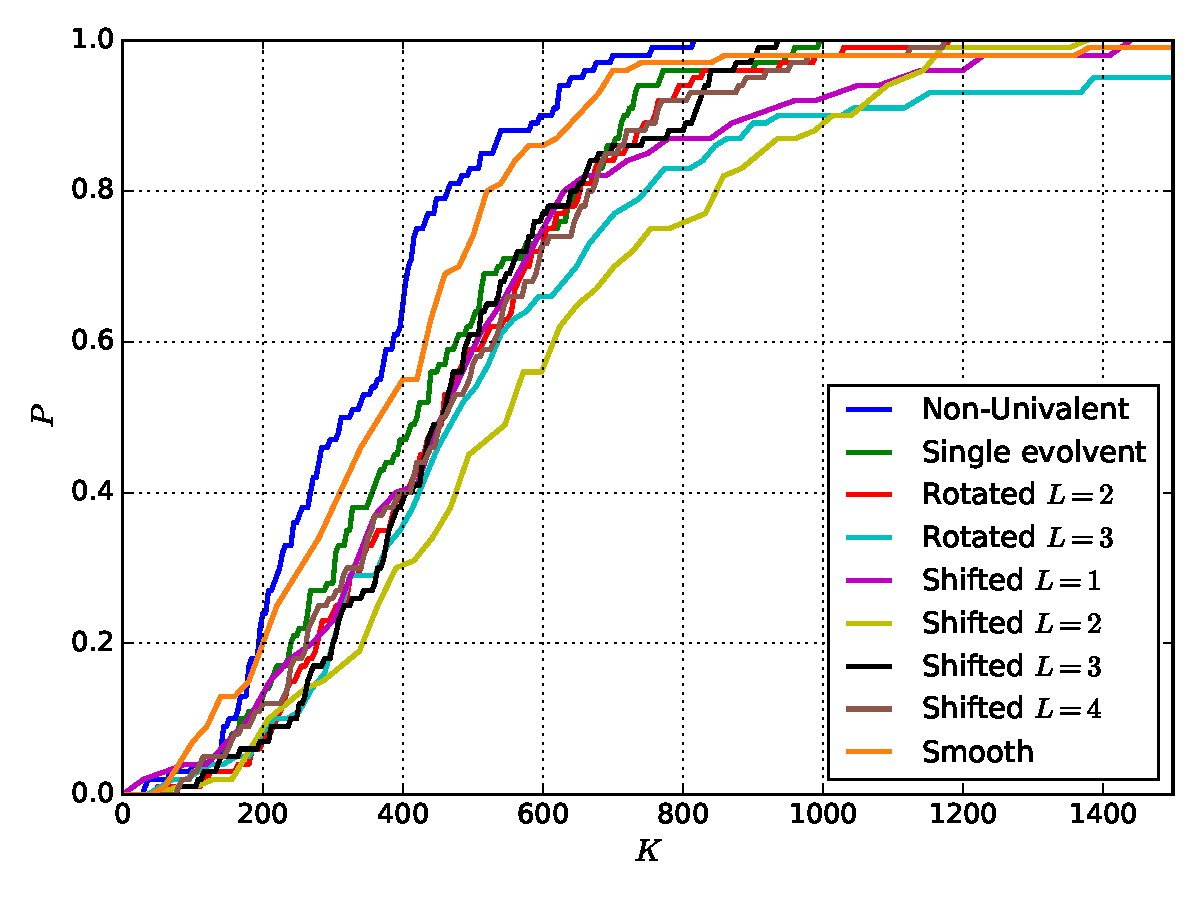
\includegraphics[width=0.95\textwidth]{../gklsS2d/opt_point/gklsS2d_opt_pt_op.pdf}
  \caption{gklsS2d, остановка по попаданию в окрестность, минимальное значение $r$}
  \label{fig:}
\end{figure}

\begin{figure}[H]
  \center
  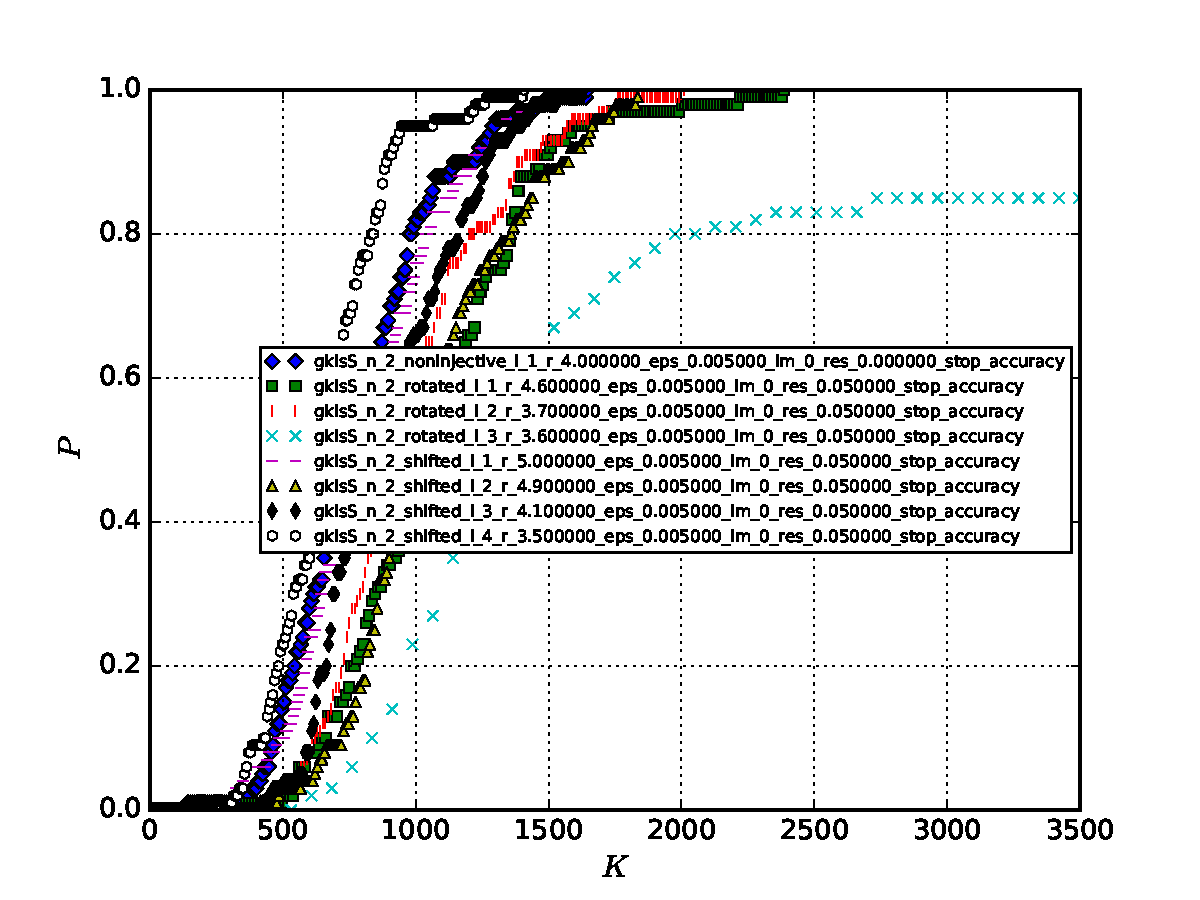
\includegraphics[width=0.95\textwidth]{../gklsS2d/accuracy/gklsS2d_acc_op.pdf}
  \caption{gklsS2d, остановка по точности, минимальное значение $r$}
  \label{fig:}
\end{figure}

\begin{figure}[H]
  \center
  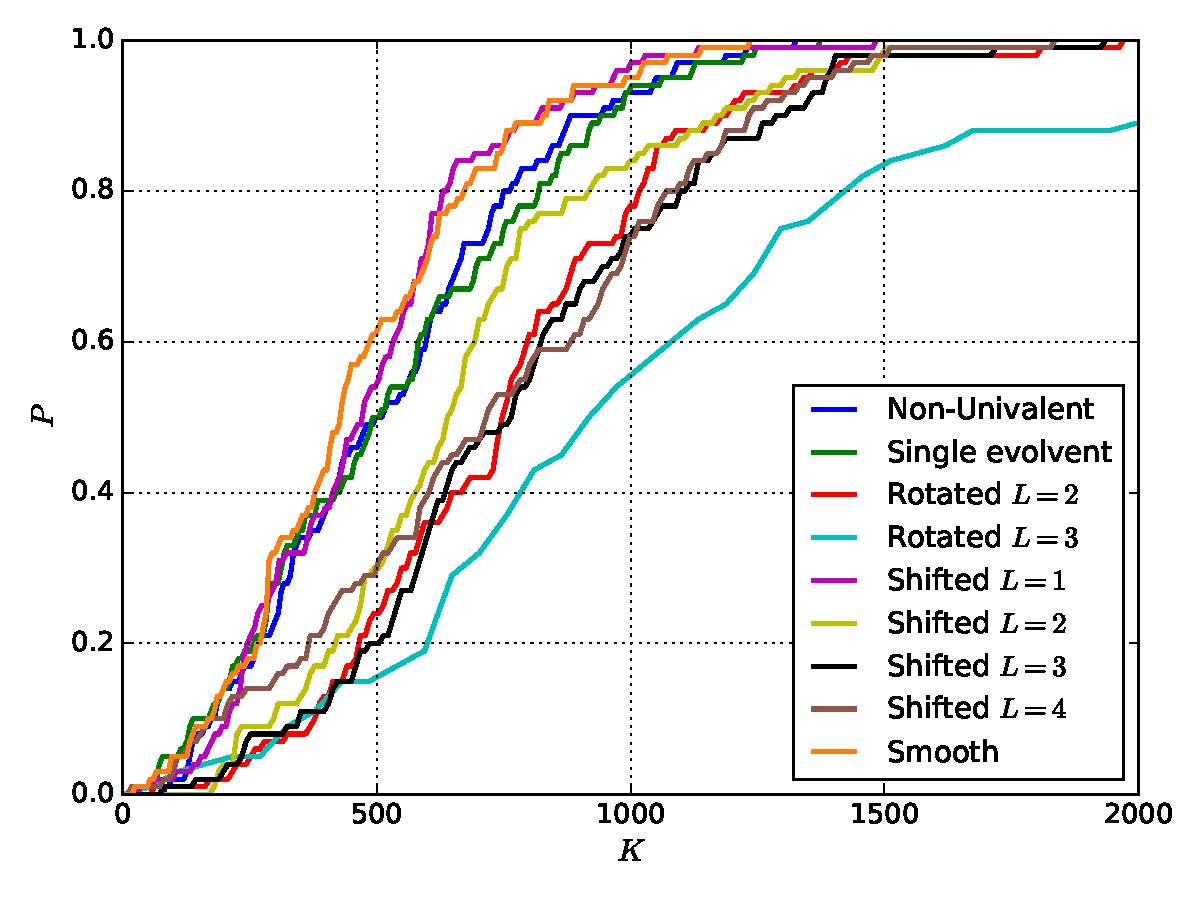
\includegraphics[width=0.95\textwidth]{../gklsS2d/same_r/opt_point/gklsS2d_same_r_opt_pt_op.pdf}
  \caption{gklsS2d, остановка по попаданию в окрестность, $r=5.0$}
  \label{fig:}
\end{figure}

\begin{figure}[H]
  \center
  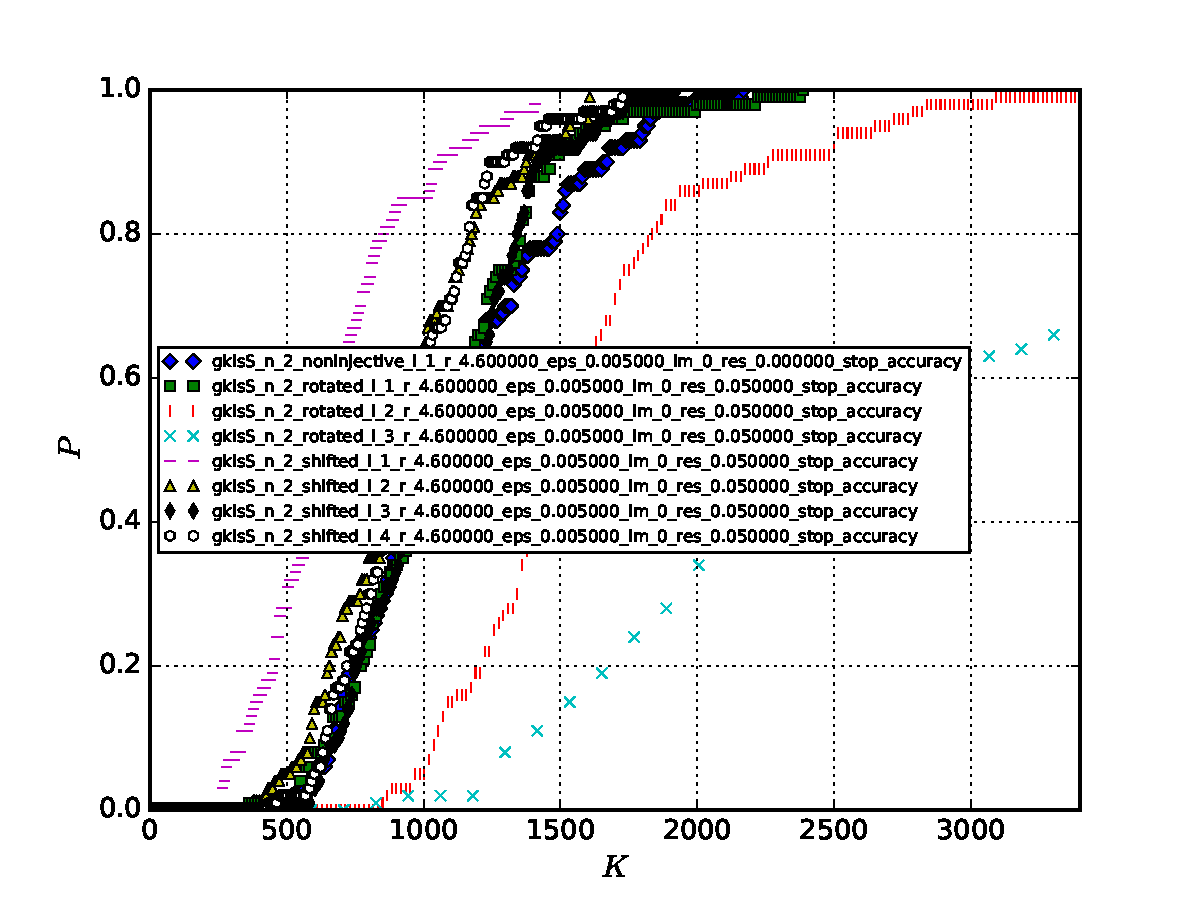
\includegraphics[width=0.95\textwidth]{../gklsS2d/same_r/accuracy/gkls2d_same_r_acc_pt_op.pdf}
  \caption{gklsS2d, остановка по точности, $r=4.6$}
  \label{fig:}
\end{figure}

\subsubsection{Класс gklsH2d}



\subsubsection{Класс gklsS3d}

\subsection{Среднее количество вычислений целевой функции}

\section{Предварительные выводы}


\end{document}
